
%%%%%%%%%%%%%%%%%%%%%%%%%%%%%%%%%%%%%%%%%%%%%%%%%%%%%%%%%%%%%%%%%%%%%%%
\section{Introduction}

By a curious coincidence, the typical escape velocity of massive
galaxies -- of order a few hundred km/s -- is such that $v_{\rm
  esc}^2/c^2$, expressed as an angular distance, is comparable to the
apparent sizes of galaxies at cosmological distances.  This
coincidence is fortunate, because it makes the gravitational lensing
deflection angle of distant galaxies ($\alpha\sim 2v_{\rm esc}^2/c^2$)
comparable to their size on the sky. As a result, strong lensing by
galaxies produces images that probe their host dark matter halos,
providing a useful tool to understand galaxy formation.  While there
is a general consensus about the basic mechanisms at play, involving
gravitational collapse, fragmentation, and mergers of dark-matter
clumps, into which gas fell, cooling through radiative processes to
form dense clouds and eventually stars, there is much debate about the
details \citep[for a summary, see][]{2012RAA....12..917S}.  In
particular, the nature of dark matter remains mysterious: most
researchers take it to be a collisionless non-relativistic fluid (cold
dark matter or CDM) readily studied by simulations \citep[for example,
  the influential Millennium
  simulation,][]{2005Natur.435..629S}. However, alternative scenarios,
where dark matter has exotic dynamical properties
\citep{2010MNRAS.405...77S,2016ApJ...818...89S}, or is not really
matter at all, but a modification of gravity
\citep{2016PhRvL.117t1101M}, have also been considered.

All this motivates the use of strong gravitational lensing over galaxy
scales to study the mutual dynamics of dark matter, gas and stars.
Several studies in recent years have done so \citep[see,
  e.g.,][]{2009ApJ...703L..51K,2011ApJ...740...97L,2012MNRAS.424..104L,
  2016MNRAS.459.3677L,2016MNRAS.456..870B} but it is desirable to
enlarge the samples from tens of lensing galaxies to thousands.  Doing
so requires both finding more lenses and also modelling their mass
distribution.  Recent searches through the CFHT Lens Survey
\citep[CFHTLS,][]{2012MNRAS.427..146H} using arc-finders
\citep[e.g.,][]{2012ApJ...749...38M,2014A&A...567A.111M,2014ApJ...785..144G,2017arXiv170401585S}
by either machine learning methods 
\citep[e.g.,][]{2016A&A...592A..75P,2017arXiv170302642L} or visual
inspection by citizen-science volunteers through the \SW project 
\citep{2016MNRAS.455.1191M} have, between them, discovered an average
of four lenses per square degree, so one can be optimistic about
finding many thousands of lenses in the next generation of wide-field
surveys, from ground-based surveys such as LSST in the optical window
and SKA in radio, to space-based missions such as Euclid and WFIRST.

The expected flood of new lens discoveries will need a similarly large
modelling effort to reconstruct their mass distributions.
Lens-modelling robots have started to be developed
\citep{2017arXiv170807377N,2017arXiv170808842H} but so far are able to
handle only very clean systems.  For typical lenses, human input is
still needed.  With that in mind \cite{2015MNRAS.447.2170K} developed
a new modelling strategy, implemented as the SpaghettiLens system.
The idea is to collaborate with experienced members of the
citizen-science community, who have already participated in lens
discovery through \SW, as well as several other projects involving
astronomical data.  The system was tested on a sample of simulated
lenses, which were part of the training and testing set in \SW.

This paper follows up that study by applying SpaghettiLens to
candidates discovered through \SW.  We present results from
the modelling of 58 of the 59 lens candidates reported by
\cite{2016MNRAS.455.1191M}.  Each lens candidate was modelled
following a collaborative refinement process, where anyone interested
could improve the analysis by modifying an existing model or creating
a new one. Note the difference with respect to the main \SW 
project, where volunteers from a group of $\gtrsim10^4$ people make
independent contributions.  Each person is presented with a random
selection of survey-patches and invited to (in effect) vote on each.
The system estimates the skill level of each volunteer according to
test-patches interspersed with the real data, and weights their votes
accordingly \citep{2016MNRAS.455.1171M}.  There is an active forum for
volunteers, but since everyone is seeing different data samples with
minimal overlap, the forum has little if any influence on the votes.
\textcolor{red}{\bf IF: Please make sure the following is correct:}
In SpaghettiLens, the number of volunteers is significantly lower, but
the level of interaction is higher.  The resulting model represents a
consensus among contributors, as to the best that could be achieved
with the available data and software.

We emphasize that the interpretation of the results presnted here is
tentative, because the systems are lens candidates at this stage, not
secure lenses.  Moreover the candidate-lens redshifts have large
uncertainties, while the candidate-source redshifts can only be
guessed at present.  Nevertheless it is interesting to explore the
trends observed with the already available data.
%TODO there is more info about uncertainies here:
% https://arxiv.org/pdf/0811.3326.pdf

This paper is organized as follows:
Section~\ref{sec:candidates_models} introduces the candidate lenses,
their models and the diagnostics applied to them.  The following
sections elaborate on the diagnostics.  Image morphology diagnostics
are explained in Section~\ref{sec:morph} and diagnostics based on the
mass models are discussed in Section~\ref{sec:massmodels}.  Stellar masses are
presented in Section~\ref{sec:stellar-mass}, to compare stellar and
lensing masses.  Finally, section~\ref{sec:summary}
summarises and tabulates the diagnostics in Table~\ref{tab:models}.

We include three appendices devoted to various technical issues
relating to the modelling.  The online supplement gives the results
from all the modelled systems generated for all the lensing
candidates.

%%%%%%%%%%%%%%%%%%%%%%%%%%%%%%%%%%%%%%%%%%%%%%%%%%%%%%%%%%%%%%%%%%%%%%%
\section{The candidates and models}
\label{sec:candidates_models}

\SW is a citizen science gravitational lens search
\citep{2016MNRAS.455.1171M}.  Its first run searched the CFHT Legacy
Survey, a survey carried out in five optical bands
($u^*$,$g^\prime$,$r^\prime$,$i^\prime$,$z^\prime$) covering a total
area of 160\,\sqdeg divided up into four fields W1 -- W4.  The
MegaPrime camera, used for the survey, has a field of view of
1\,\sqdeg, with 0.186$^{\prime\prime}$ pixels. The flux limit of the
survey is $g^\prime<$25.6AB (5\,$\sigma$) with a typical seeing
FWHM$\sim 0.7^{\prime\prime}$ \citep{2013MNRAS.433.2545E}. The cutouts
shown to the volunteers were colour composites of the $g^\prime$,
$r^\prime$ and $i^\prime$ bands from randomly chosen regions.
The programme \citep{2016MNRAS.455.1191M} resulted in 59 new lens candidates (of which 29 are
promising  \textcolor{red}{\bf IF: why are
  they promising? explain this here).}  Moreover, 82 previously known
lens candidates were ``rediscovered''.  The candidates have broadly
similar redshifts (0.2$<$z$<$1.0), Einstein radii between 0.7 and
5\,\arcsec, and arc magnitudes between 22 and 26 \textcolor{red}{\bf
  IF: in the $g^\prime$ band?}. These properties are similar to those
found by previous robotic searches like ArcFinder and RingFinder.


\begin{figure}
  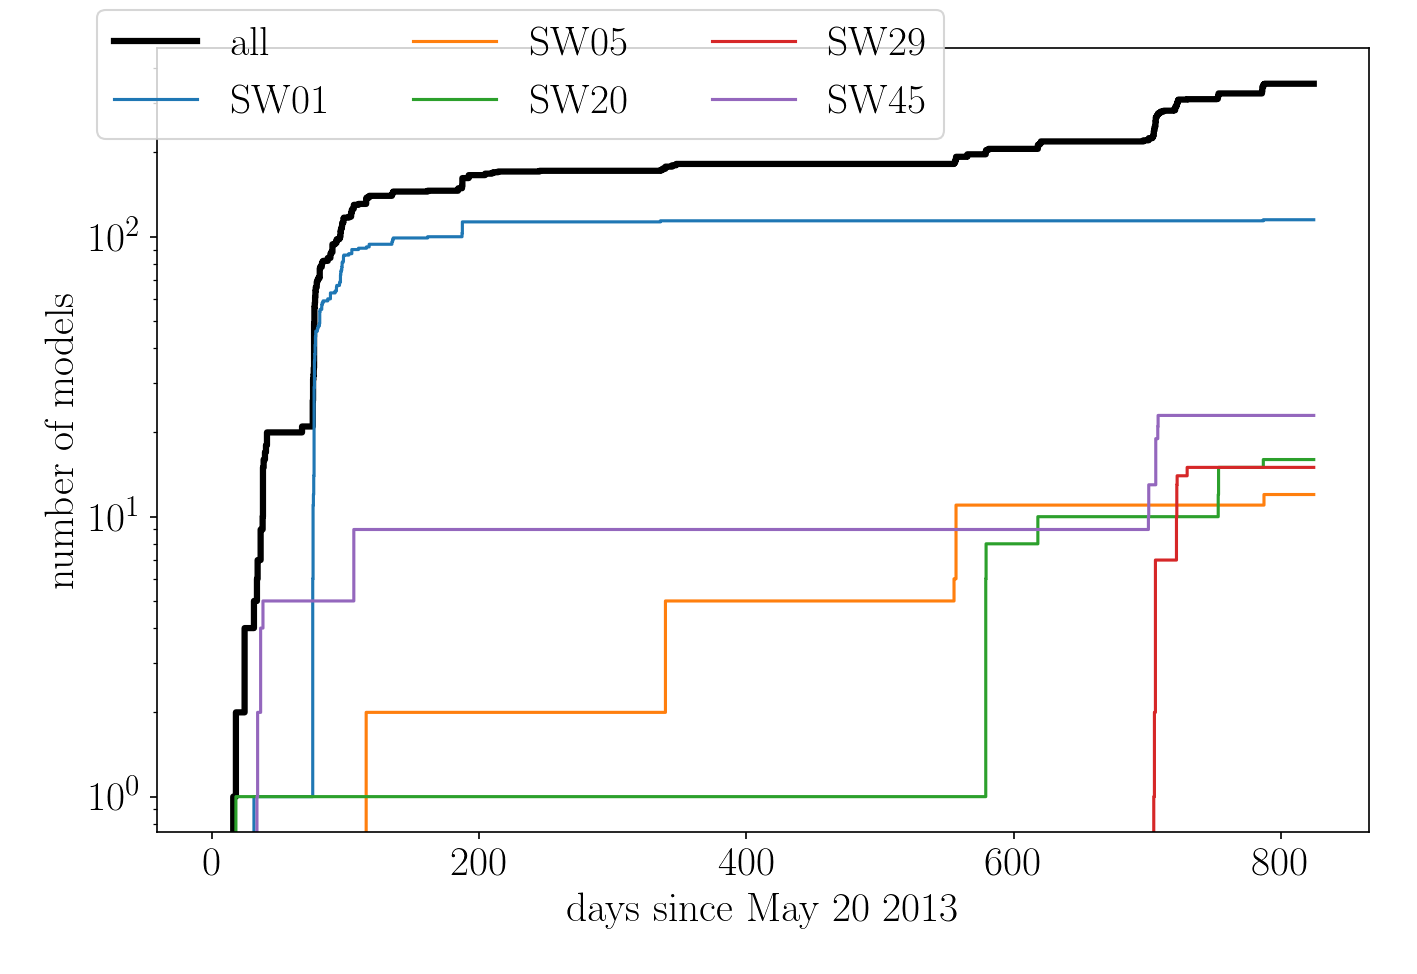
\includegraphics[width=\linewidth]{img/timelapse3}
  \caption{ Number of models generated over time in days since the
    launch of \SpL; the black line shows all models, the coloured
    lines show the five most active candidates. A total of 377 models
    were generated for 58 lens candidates, eight users contributed
    more than five models per person. }
  \label{fig:time}
\end{figure}


A first version of \SpL\footnote{\textcolor{red}{\bf IF include web
    link: {\tt http://xxx.yyy.ch}}} was launched in May 2013, while
the first run of \SW was ongoing.  Fig.~\ref{fig:time} shows the
total number of models generated since launch for our lens candidates.
A small number of volunteers started creating models of possible lens
candidates from \SW that were debated in the discussion forum.  In the
beginning of August 2013 (around day 70 since release) a modelling
challenge for the candidate later to be identified as \sw{01} was
launched.  A group of five volunteers presented their results in an
online letter \textcolor{red}{\bf REFERENCE?} about 65 days later,
converging on a set of 30 models. In April 2015 (day 700),
the first major version of \SpL was released. At the same time,
the list of identified candidates was made available \citep[as a preprint
  of][]{2016MNRAS.455.1191M}.  At this stage, the volunteers were
asked to create models for all the lens candidates that were still
missing.  The work done for candidate \sw{29} show that the
volunteers converged on a favourable model much faster, after 15
models, generated in 30 days.  The total modelling effort resulted in
a set of 377 \SpL models for all but one of the 59 \SW lens
candidates; candidate \sw{39} was not modelled by any volunteer.  Over
its runtime, the system logged eight major contributors (defined as
volunteers that generated, at least, five models).

In parallel, \citet{2015MNRAS.447.2170K} tested the system on
simulated lenses and identified some areas for improvement.  In
\S~\ref{subsec:sourcefit} we introduce fitting of the surface
brightness profile of the source.  This feature has not been included
yet in SpaghettiLens, but we carried the analysis during
post-processing for a few interesting cases.  In \S~\ref{subsec:hires}
we show that fine-grained mass maps within the central region
relieves a tendency in the earlier work for mass profiles to be too
shallow. In \S~\ref{subsec:parameter} we consider the possibility
of fitting a parametric lens model to the ensemble.
%; so far we have only been successful at extracting an Einstein radius.

We characterise each model with seven diagnostics, grouped into three
categories, whose purpose is to help identify the most likely cases of
a gravitational lens, as well as flag the most interesting candidates
for future follow-up observations. The diagnostics are as follows.

\begin{itemize}
\item Firstly we have diagnostics based on morphology.
  Section~\ref{sec:morph} and Fig.~\ref{fig:splinput} explain
  this diagnostic in more detail. We consider:
\begin{enumerate}
\item Whether the images are unblended:  Distinct, unblended images are
  an advantage in modelling, although not essential.
\item Whether all images are discernible.  The topography of an
  arrival-time surface, as encoded by a spaghetti diagram, may require
  more images than are visible, in which case the modeller has to
  insert conjectural image positions.
\item Whether the lens is isolated.
\item The image morphology concisely described: double or quads,
  further sub-categorised to indicate the elongation direction of the
  lensing mass.
\end{enumerate}
\item Secondly we have mass models, covered in Section~\ref{sec:massmodels}.
  We assess the following points:
\begin{enumerate}
\setcounter{enumi}{4}
\item Whether the mass map is reasonable (see Fig.~\ref{fig:kappa}).
\item Whether the arrival-time surface and synthetic image are
  plausible. In particular, an unsatisfactory model is flagged when 
  additional images are implied in regions
  where they are not observed (see Figs.~\ref{fig:arriv}, \ref{fig:synth} \ref{fig:encl}).
\end{enumerate}
\item Thirdly, whether the total implied lensing mass determined from
  the lens model is plausible, given the photometry of the lensing
  galaxy.  In this work we define the lensing mass as the sum of all
  mass tiles in the model.  These mass tiles reach out to typically
  twice the radius of the outermost image.
  Section~\ref{sec:stellar-mass} explains how we compare the lensing
  (i.e. total) mass with the stellar mass. Naturally, the lensing
  mass should be somewhere between the stellar mass (lower bound)
  and the total halo mass (upper bound).
\begin{enumerate}
\setcounter{enumi}{6}
\item We then introduce a so-called halo index ($\haloindex$), that
  quantifies how the lensing mass compares with these two
  constraints (see Fig.~\ref{fig:stelmass}).
\end{enumerate}
\end{itemize}






